\documentclass{standalone}

\begin{document}

Our final product thus far has been able to not only achieve the majority of the desired lensing calculations, but we were able to also implement these effects onto real images.
Examples of these visualisations can be seen in Fig.(\ref{fig:example1}) and (\ref{fig:example2}).
Both of these examples demonstrate the current robustness of gravitational lensing even for observers very near the event horizon of a black hole.

In Fig.(\ref{fig:lenscomparison}), we demonstrate the varying effectiveness of the different lensing techniques that are available in our program.
Another aspect of Fig.(\ref{fig:lenscomparison}) to note is the difference in the shapes of the graphs formed by both variants of the exact lensing equation.
We expected the only difference between the two methods would be the computation time, but the fact that they result in different graphs suggests that the \python{scipy.integrate.quad} method evaluates differently between the two approaches and discovering the cause of this may be a difficult venture.

\begin{figure*}
  \caption{\label{fig:example1}
    Final result of applying the explicit Schwarzschild lensing map on a sample image using a Schwarzschild space-time defined by $M=1.0$ and $r_O=10M$.
    In this example, one can easily see the problematic image tearing at the $\pi/2$ and $-\pi/2$ meridians.
  }
  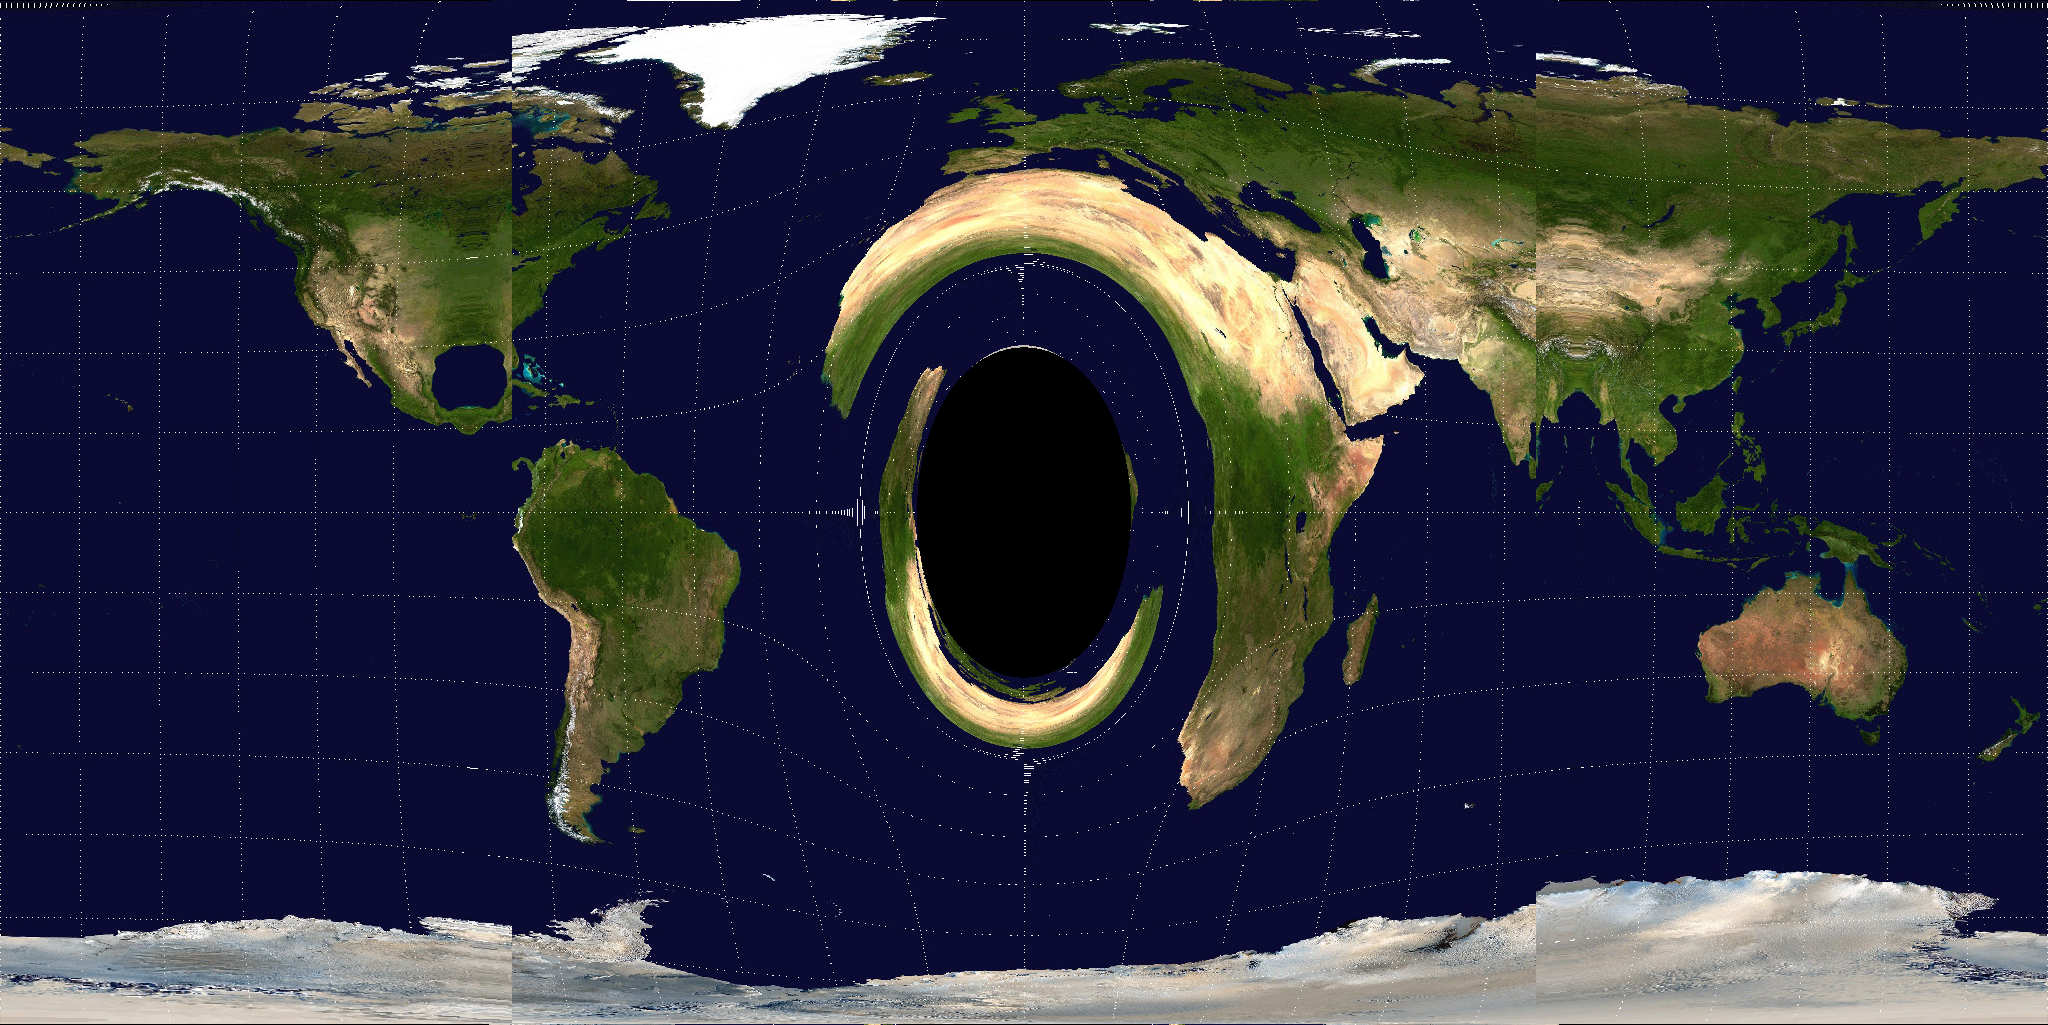
\includegraphics[width=\textwidth]{example_lens1}
\end{figure*}

\begin{figure*}
  \caption{\label{fig:example2}
    Second example of a generated Schwarzschild lensing map using the same space-time as in Fig.(\ref{fig:example1}) but at a radius of $r_O=\SI{2.5}{\kilo\meter}$, which is significantly closer to the event horizon.
    The accuracy of this result hasn't yet been scrutinized, however the overall converging of the observer's sky to the point at $\phi=0$ is to be expected.
  }
  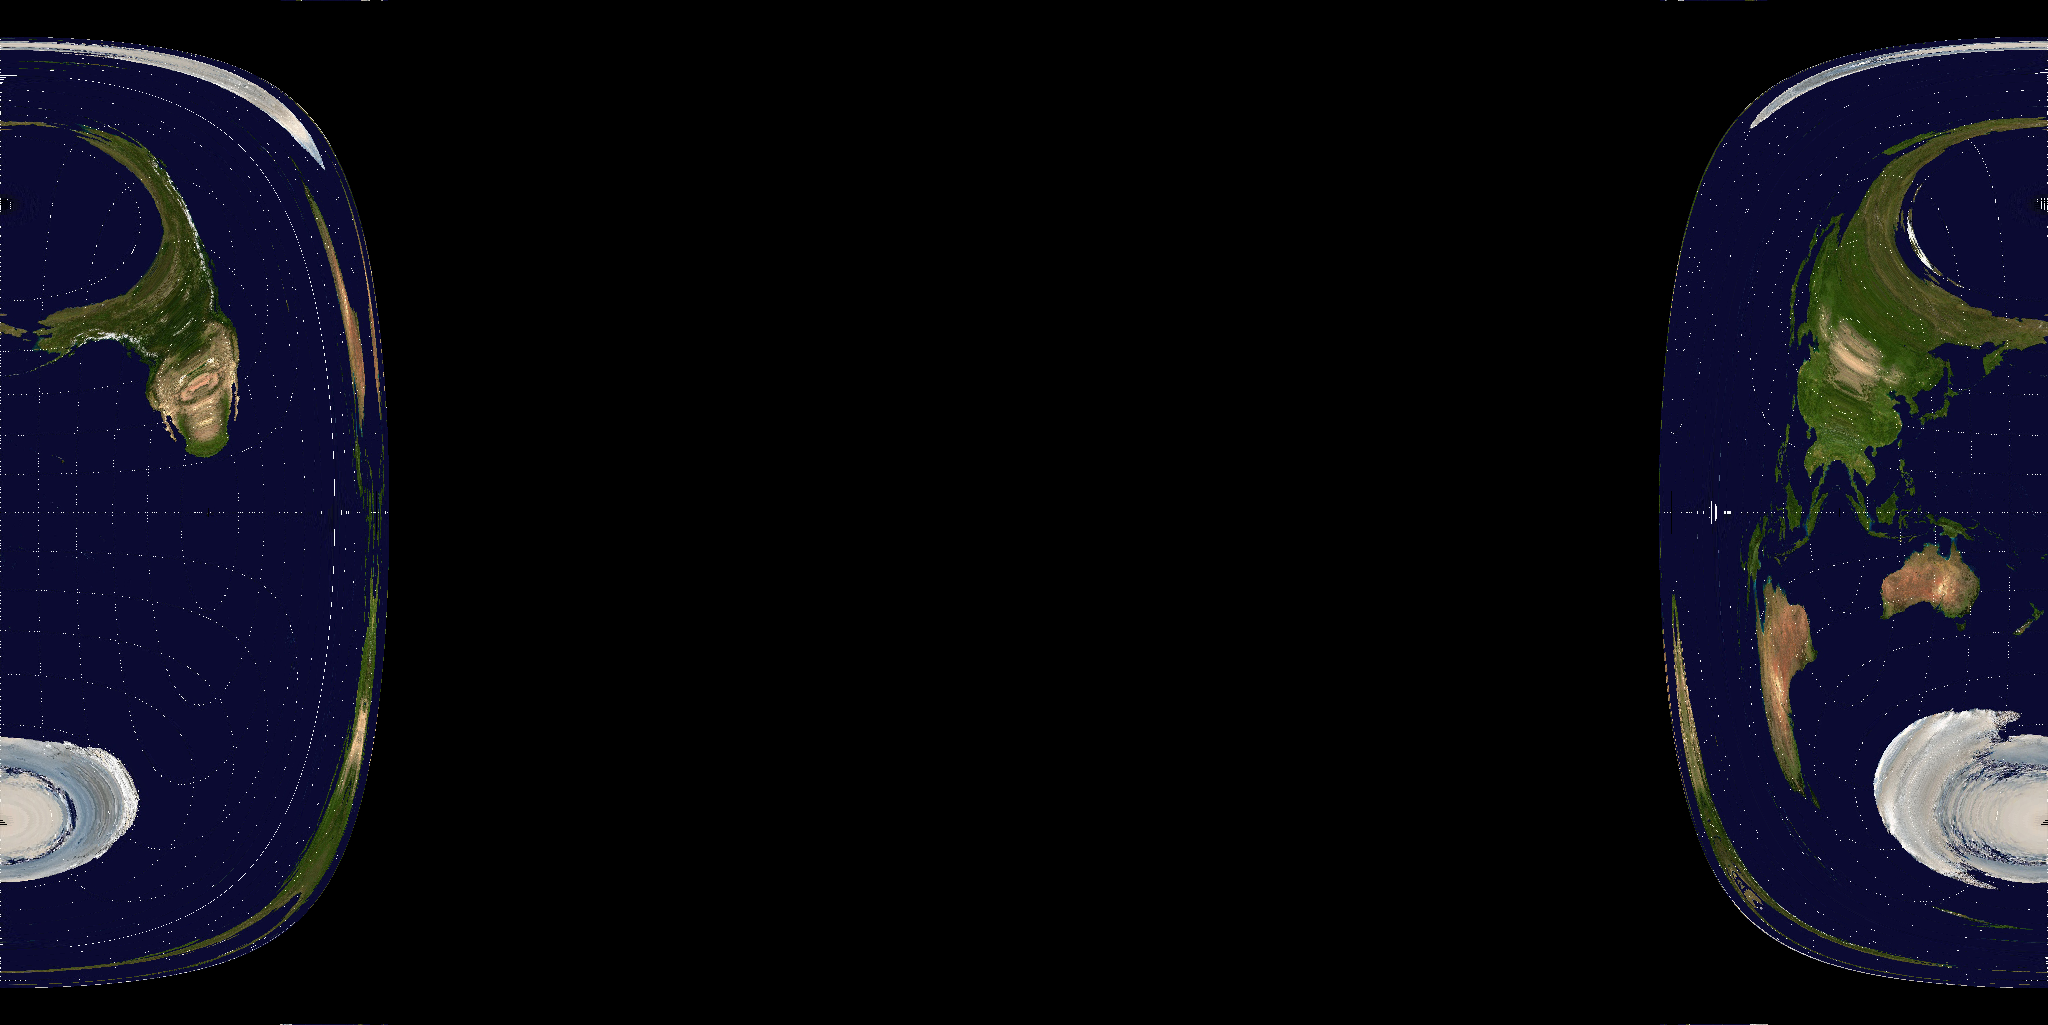
\includegraphics[width=\textwidth]{example_lens2}
\end{figure*}

\begin{figure*}
  \caption{\label{fig:lenscomparison}
    Comparison between the three levels of generality in the Schwarzschild lensing equation, with the resultant angles shifted vertically by a factor of $\pi$ for clarity.
    The first graph accentuates the differences between the methods near the singularity, while the latter graph shows how the errors of the first decrease as the radius of the observer increases.
  }
  \begin{tabular}{c}
    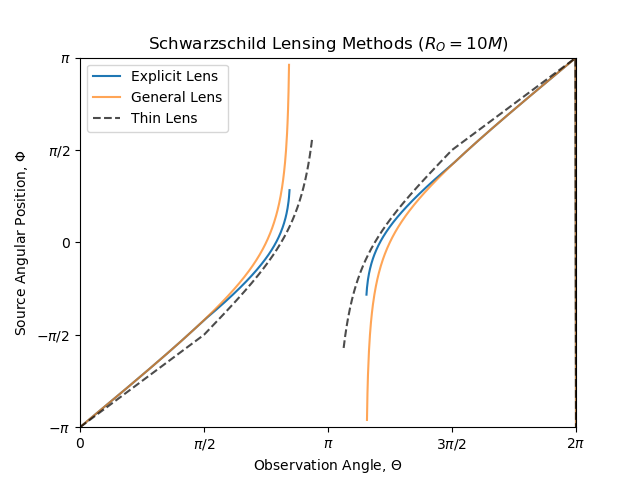
\includegraphics[width=.75\textwidth]{sc_lensing_near}\\
    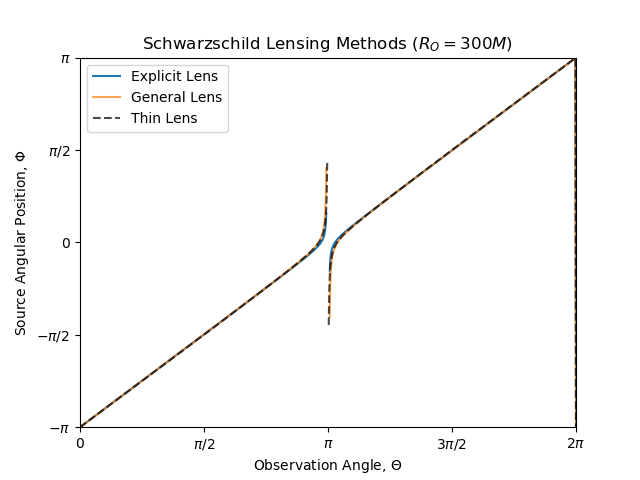
\includegraphics[width=.75\textwidth]{sc_lensing_far}
  \end{tabular}
\end{figure*}

\end{document}
